\documentclass{article}

\usepackage{arxiv}

\usepackage[utf8]{inputenc} % allow utf-8 input
\usepackage[T1]{fontenc}    % use 8-bit T1 fonts
\usepackage{lmodern}        % https://github.com/rstudio/rticles/issues/343
\usepackage{hyperref}       % hyperlinks
\usepackage{url}            % simple URL typesetting
\usepackage{booktabs}       % professional-quality tables
\usepackage{amsfonts}       % blackboard math symbols
\usepackage{nicefrac}       % compact symbols for 1/2, etc.
\usepackage{microtype}      % microtypography
\usepackage{graphicx}

\title{Automatically drawing vegetation classification maps using digital time-lapse cameras in alpine ecosystems}

\author{
    Ryotaro Okamoto
    \thanks{\url{https://github.com/0kam}}
   \\
    Doctoral Program in Biology \\
    University of Tsukuba \\
  1-1-1 Tennodai, Tsukuba, Ibaraki 305-8577 Japan. \\
  \texttt{\href{mailto:okamoto.ryotaro.su@alumni.tsukuba.ac.jp}{\nolinkurl{okamoto.ryotaro.su@alumni.tsukuba.ac.jp}}} \\
   \And
    Reiko Ide
   \\
    Earth System Division \\
    National Institute for Environmental Studies, \\
  16-2 Onogawa, Tsukuba, Ibaraki 305-8506 Japan \\
  \texttt{\href{mailto:ide.reiko@nies.go.jp}{\nolinkurl{ide.reiko@nies.go.jp}}} \\
   \And
    Hiroyuki Oguma
   \\
    Biodiversity Division \\
    National Institute for Environmental Studies, \\
  16-2 Onogawa, Tsukuba, Ibaraki 305-8506 Japan \\
  \texttt{\href{mailto:oguma@nies.go.jp}{\nolinkurl{oguma@nies.go.jp}}} \\  
  }


% tightlist command for lists without linebreak
\providecommand{\tightlist}{%
  \setlength{\itemsep}{0pt}\setlength{\parskip}{0pt}}

% From pandoc table feature
\usepackage{longtable,booktabs,array}
\usepackage{calc} % for calculating minipage widths
% Correct order of tables after \paragraph or \subparagraph
\usepackage{etoolbox}
\makeatletter
\patchcmd\longtable{\par}{\if@noskipsec\mbox{}\fi\par}{}{}
\makeatother
% Allow footnotes in longtable head/foot
\IfFileExists{footnotehyper.sty}{\usepackage{footnotehyper}}{\usepackage{footnote}}
\makesavenoteenv{longtable}


\usepackage{amsmath}
\usepackage{nicefrac}
\setlength{\parindent}{10.5pt}
\usepackage{booktabs}
\usepackage{longtable}
\usepackage{array}
\usepackage{multirow}
\usepackage{wrapfig}
\usepackage{float}
\usepackage{colortbl}
\usepackage{pdflscape}
\usepackage{tabu}
\usepackage{threeparttable}
\usepackage{threeparttablex}
\usepackage[normalem]{ulem}
\usepackage{makecell}
\usepackage{xcolor}
\begin{document}
\maketitle

%TC:ignore
\begin{abstract}
Alpine ecosystems are particularly vulnerable to climate change. Monitoring the distribution of alpine vegetation is required to plan practical conservation activities. However, conventional field observations and satellite remote sensing are difficult in terms of coverage and frequency in alpine areas. Ground-based time-lapse cameras have been used to observe the regions' snowmelt and vegetation phenology and have significant advantages in terms of cost, resolution, and frequency. However, they have not been used in research monitoring the distribution patterns of vegetation. This study proposes a novel method for drawing georeferenced vegetation classification maps from ground-based imagery of alpine regions. Our approach had two components: vegetation classification and georectification. The proposed vegetation classification method uses a pixel time series acquired from fall images to utilize the fall leaf color patterns. We demonstrated that the performance of the vegetation classification can be improved by using time-lapse imagery and a Recurrent Neural Network. We also developed a novel method to accurately transform ground-based images into georeferenced data. We propose the following approaches: 1) an automated procedure to acquire Ground Control Points; and 2) a camera model that considers lens distortions for accurate georectification. We demonstrated that the proposed approach outperforms conventional methods, in addition to achieving sufficient accuracy to observe the vegetation distribution on a plant-community scale. The evaluation revealed an F1 score and root-mean-square error of 0.937 and 3.4 m in the vegetation classification and georectification, respectively. Our results highlight the potential of inexpensive time-lapse cameras to monitor the distribution of alpine vegetation. The proposed method can significantly contribute to the effective conservation planning of alpine ecosystems.
\end{abstract}
%TC:endignore

\keywords{
    alpine ecosystem
   \and
    deep learning
   \and
    ecosystem monitoring
   \and
    time-lapse camera
  }

\hypertarget{introduction}{%
\section{Introduction}\label{introduction}}

The effects of climate change on terrestrial ecosystems are particularly severe in alpine regions, and the consequences have already been documented globally. (\cite{IPCC2007}, \cite{Gottfried2012NatClimChange}, \cite{IPCCSR2019HM}). Alpine vegetation depends on severe conditions such as low temperatures and long snow-covered periods. Alpine areas have unique species that are adapted to such extreme environments. Several studies have reported that recent global climatic changes, such as increasing temperatures and reduced periods of snow cover, have accelerated the invasion of non-native species into alpine areas (see \cite{Alexander2016AlpBotany}). In the Taisetsu Mountains, northern Japan, dwarf bamboo (\emph{Sasa kurilensis}) has invaded alpine snow meadows, possibly driven by an extension of the snow-free period (\cite{Kudo2011EcoEvo}). Researchers have also predicted a decrease in suitable habitats for alpine snow meadows in this area (\cite{Amagai2022AVS}). Climate change has also affected the growth and phenology of native species. For example, the growth of dwarf pine (\emph{Pinus pumila}), a dominant species in Japanese alpine regions, has been affected by climatic conditions such as temperature and snowmelt timing (\cite{Amagai2015EcoRes}). In addition, such changes vary depending on the species and microhabitats (\cite{Kudo2010AAA}). Understanding and predicting changes in alpine vegetation requires a monitoring method scalable to a wide range with high spatiotemporal resolution.

Previous studies on alpine ecosystems have relied heavily on field observations; however, it is difficult to cover large areas in alpine regions due to poor accessibility and severe weather. Additionally, variance in alpine plant phenology complicates this problem. Strictly limited by snow cover, the growing season of alpine plants is typically very short, and their phenology varies greatly across years and microtopography (\cite{Kudo1991AAR}). Thus, it is difficult to plan observations by predicting plant phenology, rendering continuous observations over several months necessary. Satellite, airborne, and Unmanned Aerial Vehicle (UAV) remote-sensing methods appear to be alternatives. However, satellite imagery of alpine areas is rarely available because of cloud cover, and the spatial resolution is insufficient to observe vegetation changes at the plant community scale. Airborne imagery can be used to obtain high-resolution data, but frequent monitoring is restricted by its cost. Although UAV methods have become cost-effective tools for ecological monitoring (\cite{Baena2017PLOSONE}), continuous monitoring with UAVs in alpine regions is difficult because of severe weather.

Researchers have utilized automated digital time-lapse cameras mounted on the ground to monitor green-leaf phenology in forests (\cite{Richardson2009EcolAppl}), grasslands (\cite{Browning2017RemSen}), and alpine meadows (\cite{IdeOguma2013EcolInfom}). Unlike satellite imagery, ground-based cameras provide images free of cloud and atmospheric effects. In addition, they can obtain high-resolution (i.e., sub-meter scale) and frequent (i.e., daily or hourly) images at a low cost. Most previous studies using such cameras have calculated the phenology index (e.g., excess greenness, \cite{Woebbecke1995ASAE}) by setting some regions of interest (ROI) in the images. Few studies have utilized such images to monitor vegetation distributions. This is possibly because applying such time-lapse imagery to monitor vegetation distribution has two technical challenges. The first limitation is the spectral sensitivity of the camera. Ordinary digital cameras can only obtain three bands in the visible range (Red, Green, and Blue), rendering the accurate classification of vegetation difficult. However, researchers have reported that using multi/hyperspectral data, particularly in infrared regions, improves the accuracy of vegetation classification (\cite{Thenkabail2004RemSenEnv}, \cite{Schmidt2003RemSenEnv}). The second limitation is the availability of images in geospatial analyses. As digital time-lapse cameras are mounted on the ground, transforming the images into geospatial data (e.g., orthoimages; this process is called georectification) is challenging. That is, even if we classify vegetation from such images, we cannot quantitatively measure and analyze it using Geographic Information System (GIS) tools. Georectification is essential for utilizing time-lapse cameras in conservation planning.

This study proposes an automated method for drawing vegetation classification maps using a digital time-lapse camera by solving the two above-mentioned challenges. We solved the first challenge by using time-lapse images to classify vegetation. Fall leaf phenology, which varies among species, was used for classification. We demonstrated the effectiveness of such phenological information for vegetation classification. A novel georectification method for ground-based images was developed to address the second challenge. Using the proposed procedure, we generated a vegetation classification map from the time-lapse images of the Japanese Alps. Our approach enabled us to continuously monitor vegetation distribution and its changes at a plant-community scale, covering broad areas at a low cost.

\hypertarget{materials-and-methods}{%
\section{Materials and methods}\label{materials-and-methods}}

The proposed method comprises three steps:
\begin{enumerate}
\def\labelenumi{\arabic{enumi}.}
\tightlist
\item
Image-to-image alignment for correcting the movements of the camera.
\item
Vegetation classification for classifying each pixel into vegetation categories.
\item
Georectification for transforming vegetation classification results into geospatial data.
\end{enumerate}

Fig. \ref{fig:diagram} shows the overview of the entire process. The proposed method requires a training dataset to train the vegetation classification model, and, for the georectification process, a Digital Elevation Model (DEM), and a georectified airborne/satellite image that covers the camera's field of view.



\begin{figure}
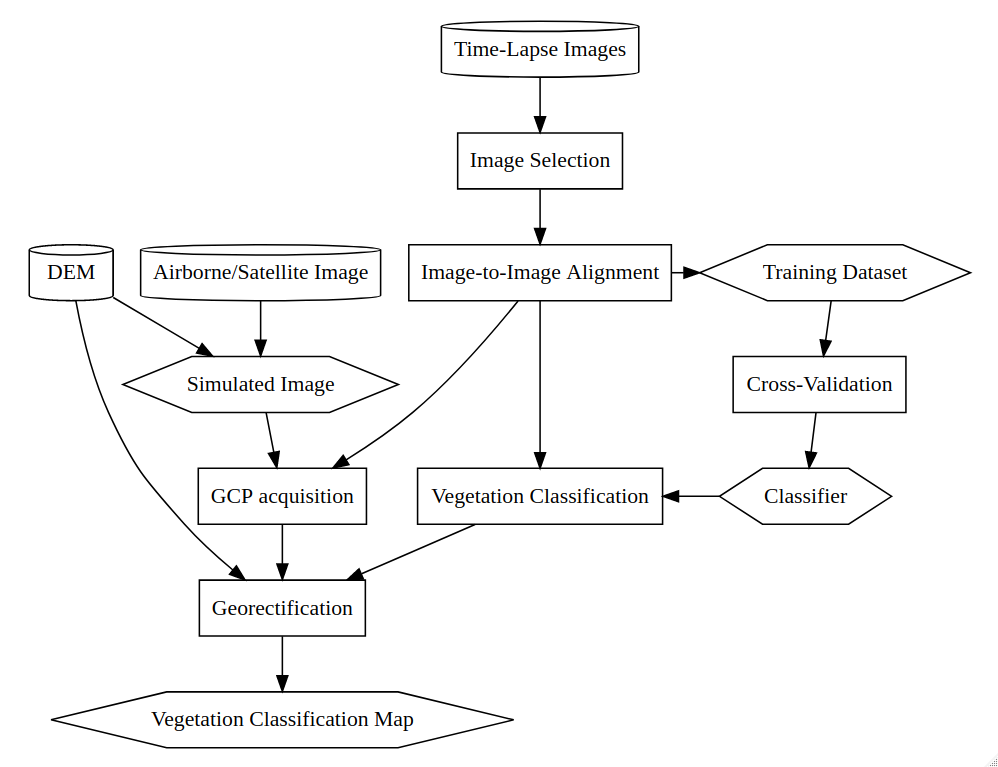
\includegraphics[width=0.8\linewidth]{paper_files/figures/diagram} 
\caption{An overview of the proposed procedure. The cylinders, boxes, and hexagons represent the source data to prepare, procedures, and deliverables, respectively.}
\label{fig:diagram}
\end{figure}

\hypertarget{time-lapse-image-acquisition}{%
\subsection{Time-lapse image acquisition}\label{time-lapse-image-acquisition}}

Our approach is intended for digital time-lapse images of alpine landscapes. In this study, we demonstrated the approach using time-lapse images of a Japanese alpine region owned by the National Institute for Environmental Studies, Japan (NIES). All images are publicly available on the NIES webpage (\url{https://db.cger.nies.go.jp/gem/ja/mountain/statWeusedtml?id=2}). In 2010, NIES installed a digital time-lapse camera (EOS 5D MK2, Canon Inc., 21 M pixels) at a mountain lodge (Murodo-sanso; approximately 2450 m a.s.l. and above the forest limit), located at the foot of Mt. Tateyama (3015 m a.s.l.), in the northern Japanese Alps (Fig. \ref{fig:map}). The area is designated as a restricted zone within the Chubusangaku National Park. The images were taken hourly, from 6 a.m. to 7 p.m., in JPEG format. The camera's field of view (FoV) includes Mt. Tateyama, which ranges from approximately 2350–3015 m a.s.l. in elevation. The pixel size on the ground was approximately 0.5 m at the ridge, approximately 1 km from the camera. The area has a complex mosaic-like vegetation structure because of its topography and climate, including rocks, cliffs, curls, moraines, and heavy winter snow. From April–November, the camera recorded the snowmelt and seasonal phenology of evergreen (e.g., \emph{Pinus pumila}) and deciduous (\emph{Sorbus} sp., \emph{Acer tschonoskii}) dwarf trees, dwarf bamboos (e.g., \emph{Sasa kurilensis}), alpine shrubs, and herbaceous plants (e.g., \emph{Vaccinium ovalifolium}, \emph{Geum pentapetalum}, and \emph{Nephrophyllidium crista-galli}).

\begin{figure}
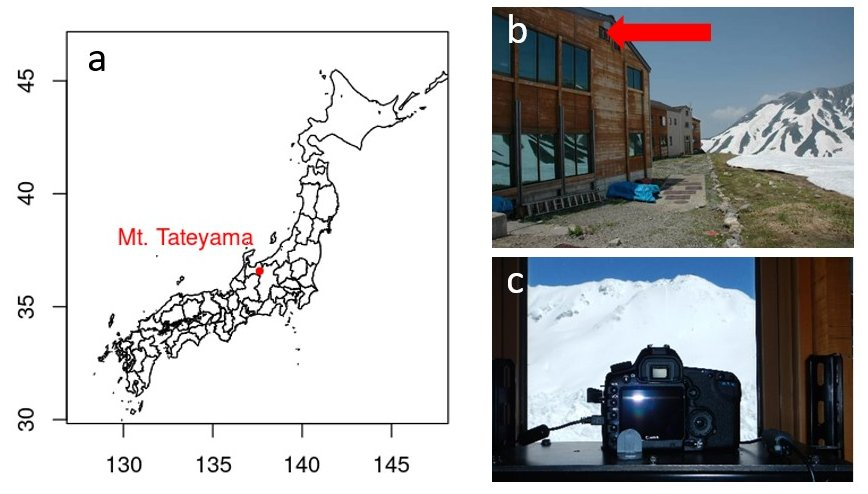
\includegraphics[width=1\linewidth]{paper_files/figures/Slide3} \caption{The location of the camera. (a) The location of Mt. Tateyama. (b) The installation point of the camera in Murodo-sanso lodge. (c) The camera (EOS 5D MK2, Canon Inc.)}\label{fig:map}
\end{figure}

\hypertarget{preprocessing}{%
\subsection{Preprocessing}\label{preprocessing}}

\hypertarget{image-selection}{%
\subsubsection{Image selection}\label{image-selection}}

Initially, we selected seven images with good weather from late summer to late fall (25 Aug; 5, 12, 20, and 26 September; 3 and 10 October) in 2015. To avoid the effects of shadows, we selected images from 11:00 a.m. to 2:00 p.m. As the temporal patterns of fall foliage coloration vary among species, this season is suitable for classifying vegetation. While acquiring a series of images is expensive with UAVs and airborne imagery, time-lapse cameras are particularly good at observing temporal patterns of leaf color at low cost.

\hypertarget{automatic-image-to-image-alignment}{%
\subsubsection{Automatic image-to-image alignment}\label{automatic-image-to-image-alignment}}

Time-lapse images often suffer from camera movement caused by strong winds, human interference, and thermal expansion of the camera platform. As such movements can result in errors in vegetation classification and georectification, we implemented an image alignment method that aligns one (source) image to another (target) image. The software was developed using Python3 and the OpenCV4 image processing library (\url{https://opencv.org/}). We employed the feature-based alignment method used in previous studies (\cite{Hulton2020PyTrx}, \cite{Portenier2020Cryosphere}). First, we searched and matched key points between the source and the target image using the AKAZE local feature extractor (\cite{Alcantarilla2013AKAZE}) and the K-nearest neighbor matcher. Then, we searched and applied the \(3 \times 3\) homography matrix \(H\) that minimizes the distance between each pair of the matching points, using OpenCV's ``findHomography'' function:
\begin{equation}
\label{homography}
  \begin{bmatrix} 
    U' \\ V' \\ 1
  \end{bmatrix}
  =
  H
  \begin{bmatrix}
    U \\ V \\ 1
  \end{bmatrix},
\end{equation}
where \([U', V', 1]\) and \([U, V, 1]\) represent the coordinates of the matching points on the target and source images, respectively. By setting one image as the target and the others as the source, the entire time-series imagery was aligned accurately (0.654 pixels in root mean square error (RMSE) of the matching points). Finally, an input mask was applied to define the image regions that should be ignored in the following procedure, such as the sky and regions too close to the camera. This process ensures that a pixel time series reflects phenological information about the exact location, which is essential in the vegetation classification process.

\begin{figure}
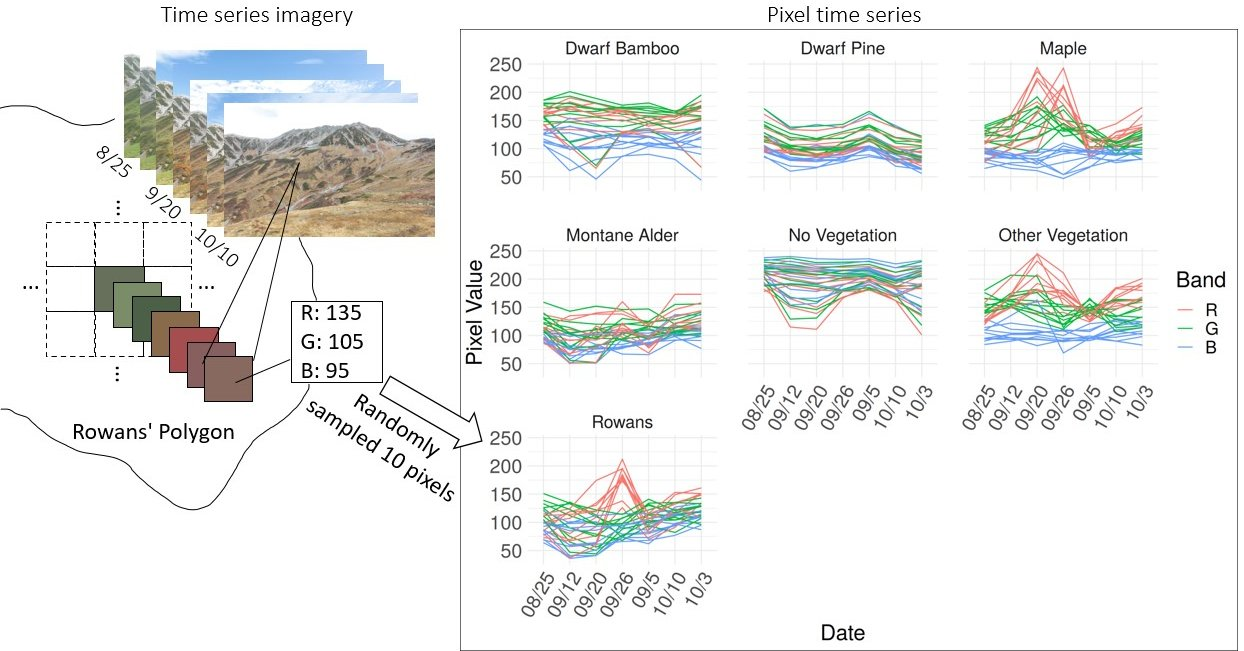
\includegraphics[width=1\linewidth]{paper_files/figures/Slide1} \caption{Pixel time series acquired from the time-lapse camera. A time series of pixel values (i.e., Red, Green, and Blue) for each pixel on the images (left) can be obtained. Since the images were taken in 8-bit JPEG format, the pixel values range from 0 to 255. The plots on the right show the pixel time series of 10 pixels randomly sampled for each class. Each line represents a pixel's value (Red, Green, or Blue, shown as the line color) sampled from manually annotated vegetation polygons that were used to train the vegetation classifier (see \ref{dataset-preparation} for more detail).  Such pixel time series reflect the fall phenology of the vegetation and vary among vegetation classes. For example, the high Red values on Maple and Rowans show the fall foliage. On the other hand, evergreen vegetation, such as Dwarf bamboo and Dwarf pine, show flat patterns in pixel values.}\label{fig:pixtimeseries}
\end{figure}

\hypertarget{vegetation-classification}{%
\subsection{Vegetation classification}\label{vegetation-classification}}

After image-to-image alignment, we stuck the images and extracted a time series of pixel values (Red, Green, and Blue, see Fig. \ref{fig:pixtimeseries}) for each pixel. Such pixel time series reflect the temporal patterns of leaf colors that vary among species. For example, Rowans (\emph{Sorbus sambucifolia, Sorbus matsumurana}), which turn red in the fall, exhibited high Red values at the end of September. Maple (\emph{Acer tschonoskii}), which turns yellow to orange and red in the fall, also has high Red values in September but with two peaks. This implies that Maple has intra-species variation in the timing of fall foliage. As deciduous plants show great interspecific variation in fall leaf phenology, researchers have used this information together with satellite imagery for vegetation classification (\cite{Son2013RemSen}, \cite{Tigges2013RemSenEnv}, \cite{Heupel2018PFG}). However, no study has applied this technique to ground-based time-lapse imagery. We implemented a Support Vector Machine- (SVM) and Recurrent Neural Network- (RNN) based vegetation classifiers and tested the effects of using the pixel time series from the ground-based imagery on the classification performance.

\hypertarget{model-architecture}{%
\subsubsection{Model Architecture}\label{model-architecture}}

We prepared two supervised models, SVM and RNN, to classify pixel time series into vegetation categories. The SVM is one of the most popular machine-learning models in remote sensing and has many applications (\cite{Mountrakis2011SVMReview}), including vegetation classification with multitemporal satellite imagery (\cite{Tigges2013RemSenEnv}). An RNN is a neural network that recurrently processes sequential or temporal steps of data to recognize their dynamics. Recurrent Neural Networks have been used in many tasks, such as speech recognition (\cite{Graves2013SpeechRNN}, \cite{Graves2014SpeechRNN}, \cite{Sak2014acousticLSTM}) and machine translation (\cite{Auli2013translationRNN}, \cite{Cho2014RNN}). Researchers have also utilized RNN for remote sensing tasks, such as land cover classification, with multitemporal satellite imagery (\cite{Ienco2017RemSenLSTM}, \cite{Sharma2018NN}). A previous study (\cite{Ienco2017RemSenLSTM}) reported that an RNN classifier outperformed an SVM classifier in terms of land cover classification accuracy. Among the many variants of RNN, we used Long Short-Time Memory (LSTM) \cite{Hochreiter1997LSTM}), which was also used in a previous study (\cite{Ienco2017RemSenLSTM}). The batch-normalization technique (\cite{IoffeSzegedy2015BatchNorm}) and GELU activation function (\cite{HendrycksGimpel2016GELU}) were employed to speed up and stabilize the model training. As a comparison, we also classified the pixels of every single image separately using SVM classifiers to test whether using multitemporal imagery improves the classification performance.

\hypertarget{dataset-preparation}{%
\subsubsection{Dataset preparation}\label{dataset-preparation}}

Each pixel time series was classified into seven vegetation classes: Dwarf Pine (\emph{Pinus pumila}), Dwarf Bamboo (\emph{Sasa kurilensis}), Rowans (\emph{Sorbus sambucifolia}, \emph{Sorbus matsumurana}), Maple (\emph{Acer tschonoskii}), Montane Alder (\emph{Alnus viridis} subsp. \emph{maximowiczii}), Other Vegetations (such as alpine shrubs and herbaceous plants), and No Vegetation. Experts prepared a training dataset for each class using open-source image annotation software (Semantic Segmentation Editor, Hitachi, \url{https://github.com/Hitachi-Automotive-And-Industry-Lab/semantic-segmentation-editor}). The prepared training dataset contained approximately 1.5 M pixels in 137 polygons, which covered approximately 7\% of the image. Each polygon was validated using a set of telephotos that overlapped with the camera's FoV. The telephotos were taken in the fall of 2014 using a Nikon D7100 camera (Nikon Corp.) with a 200 mm lens. Although we were able to observe the shape and texture of the plant community from the telephotos, some vegetation could not be identified without more detailed observation (such as of leaf shapes). We conducted a field survey in September 2022 to identify the vegetation types in these locations.

\hypertarget{experimental-settings}{%
\subsubsection{Experimental Settings}\label{experimental-settings}}

We implemented the classifiers using Python3 language. For the SVM classifier, we used the ThunderSVM library (\\ url{https://github.com/Xtra-Computing/thundersvm}) and a Radial Basis Function (RBF) kernel with a regularization parameter equal to 1.0. The gamma value of the RBF kernel was set automatically by the ``scaled`` setting of the ThunderSVM library as \(\gamma = \frac{1}{n_{features} \times V(X)}\), where \(n_{features}\) and \(V(X)\) represent the input data's dimensions and variance, respectively. The RNN classifier was developed using the PyTorch deep neural network library (\url{https://pytorch.org/}). The number of hidden dimensions was set to five. We trained the model for 200 epochs using the Rectified Adam optimizer (\cite{Liu2020RAdam}) with a learning rate of 0.001 and batch size of 500. To validate the performance of the different classifiers, we performed a 5-fold cross-validation. Each fold was stratified according to the vegetation category. As a model evaluation metric, we used the per-class F1-score, a standard metric in machine learning (\ref{f1score}). \(TP, FP, FN\) stand for the numbers of true positives, false positives, and false negatives, respectively. All the source codes are available via GitHub (\url{https://github.com/0kam/VegetationMapPaper}).

\label{f1score}
\begin{align}
\label{metrics}
  \begin{gathered}
  precision = \frac{TP}{TP + FP} \\
  recall = \frac{TP}{TP + FN} \\
  F_1 = \frac{2 \cdot precision \cdot recall}{precision + recall} \\
  \end{gathered}
\end{align}

\hypertarget{automatic-georectification}{%
\subsection{Automatic georectification}\label{automatic-georectification}}

The second challenge of utilizing time-lapse cameras in vegetation monitoring is the difficulty of georectification, that is, georeferencing and transforming images into geographic data. That is, georectification refers to aligning images onto Digital Surface Models (DSMs) so that every pixel of an image gets a geographical coordinate. This typically requires a camera model. Georectification of ground-based images has been a difficult task, which has led to the underutilization of the potentially rich information in ground-based imagery. We developed a novel method for performing this process automatically and accurately. We considered a camera as a function that transforms 3D geographical coordinates (e.g., X, Y, and Z (height) in a Universal Transverse Mercator coordinate system (UTM)) into 2D image coordinates (locations of each pixel in the image). By estimating the parameters of this function (such as camera location, pose, and FoV, one can simulate how each point of the DSM appears in the image. Georectification usually has three steps:

\begin{enumerate}
\def\labelenumi{\arabic{enumi}.}
\tightlist
\item
  Finding Ground Control Points (GCPs) in the image.
\item
  Estimating the camera parameters, such as the camera pose and FoV, using GCPs.
\item
  Projecting the image onto the DSM using the camera parameters.
\end{enumerate}

Researchers have recently developed georectification methods to use ground-based images in glaciology (\cite{Messerli2015GeoInst}, \cite{Hulton2020PyTrx}) and snow cover studies (\cite{Portenier2020Cryosphere}). Typically, Global Navigation Satellite System- (GNSS)positioned GCPs (such as GCP markers) are set before image acquisition. However, setting such markers in alpine areas is often difficult owing to their rugged topography. \cite{Portenier2020Cryosphere} tackled this problem by developing a method that uses mountain silhouettes to match an image and a DSM directly. However, this silhouette-based method has a drawback in terms of projection accuracy; it ignores lens distortion and uses only limited areas (silhouettes) of images in the GCP acquisition. To overcome this drawback, this study proposes a camera model that includes lens distortion and a novel method to acquire GCPs in a broader area than that of the silhouette-based method.

\hypertarget{modeling-and-estimating-camera-parameters}{%
\subsection{The camera model}\label{modeling-and-estimating-camera-parameters}}

In this section, we explain our camera model, which considers lens distortion. As mentioned previously, we modeled a camera as a function that transforms geographical coordinates into image coordinates. This procedure was implemented using the OpenGL framework (\url{https://www.opengl.org}) and the ModernGL Python library (\cite{moderngl}) to accelerate it using graphical processing units (GPUs). In OpenGL, this process can be separated into three steps.

\begin{enumerate}
\def\labelenumi{\arabic{enumi}.}
\tightlist
\item
  Transforming the geographical coordinates (also called the world coordinates) to the view coordinates (coordinates seen from the camera's point of view) using the camera's extrinsic parameters (i.e., the location and angles of the camera).
\item
  Distorting the view coordinates using the lens distortion parameters.
\item
  Transforming the view coordinates into the image coordinates (also called the screen coordinates) using the camera's intrinsic parameters (i.e., the camera's FoV).
\end{enumerate}

First, we transformed the geographic coordinates into view coordinates relative to the camera's position and direction. We used a \(4 \times 4\) view matrix (Eq. \ref{view_matrix}) \(M_{view}\) in this step. The view matrix represents the camera position and direction (pan, tilt, and roll):

\begin{equation}
\label{view_matrix}
  M_{view} = 
  \begin{bmatrix}
    \cos roll & -\sin roll & 0 & 0 \\
    \sin roll & \cos roll & 0 & 0 \\
    0 & 0 & 1 & 0 \\
    0 & 0 & 0 & 1 \\
  \end{bmatrix}
  \begin{bmatrix}
    1 & 0 & 0 & 0 \\
    0 & \cos tilt & -\sin tilt & 0 \\
    0 & \sin tilt & \cos tilt & 0 \\
    0 & 0 & 0 & 1 \\
  \end{bmatrix}
  \begin{bmatrix}
    \cos pan & 0 & \sin pan & 0 \\
    0 & 1 & 0 & 0 \\
    -\sin pan & 0 & \cos pan & 0 \\
    0 & 0 & 0 & 1 \\
  \end{bmatrix}
  \begin{bmatrix}
    1 & 0 & 0 & -x \\
    0 & 1 & 0 & -z \\
    0 & 0 & 1 & -y \\
    0& 0 & 0 & 1 \\
  \end{bmatrix},
\end{equation}
where \(pan, tilt, roll\) are the Euler angles of the camera pose and \(x, y, z\) are the camera location in the geographic coordinate system. Applying the view matrix \(M_{view}\) transforms the geographic coordinates \(\begin{bmatrix} X_{geo} & Z_{geo} & Y_{geo} & 1 \end{bmatrix}\) (the horizontal, vertical, and depth coordinates, respectively) into the view coordinates \(\begin{bmatrix} X_{view} & Z_{view} & Y_{view} & 1 \end{bmatrix}\) (Eq. \ref{view_tf}). In the OpenGL's view coordinate system, \(X_{view}\), \(Z_{view}\) and \(Y_{view}\) represent the horizontal, vertical, and depth positions, respectively. Note that the geographic coordinate system must be cartesian (such as the UTM coordinate systems) and not the lat/long coordinate system.

\begin{equation}
\label{view_tf}
  \begin{bmatrix} 
    X_{view} \\ Z_{view} \\ Y_{view} \\ 1 
  \end{bmatrix}
  =
  M_{view}
  \begin{bmatrix} 
    X_{geo} \\ Z_{geo} \\ Y_{geo} \\ 1 
  \end{bmatrix}
\end{equation}

Second, we distorted the view coordinates to simulate lens distortion. We modeled the lens distortion (Eq. \ref{dist_model}) based on \cite{Weng1992CameraCalib} and OpenCV's implementation (\url{https://docs.opencv.org/4.x/d9/d0c/group__calib3d.html}), where \(X_{norm}\) and \(Z_{norm}\) are the \(Y\)-normalized view coordinates. This model distorts the point locations according to the distance from the center of the image. Our model includes radial (\(k1\)\textasciitilde{}\(k6\)), tangential (\(p1\), \(p2\)), thin prism (\(s1\)\textasciitilde{}\(s4\)) distortion, and unequal pixel aspect ratios (\(a1\), \(a2\)). See \cite{Weng1992CameraCalib} for details on lens distortion modeling.

\begin{gather}
\label{dist_model}
  \begin{gathered}
  X_{norm} = \frac{X_{view}}{Y_{view}} \\
  Z_{norm} = \frac{Z_{view}}{Y_{view}} \\
  r^2 = {X_{norm}}^2 + {Z_{norm}}^2 \\
  \begin{bmatrix}
    X_{dist\_norm} \\ 
    Z_{dist\_norm} \\
  \end{bmatrix} 
  = 
  \begin{bmatrix} 
    X_{norm} \frac{1 + k_1 r^2 + k_2 r^4 + k_3 r^6}{1 + k_4 r^2 + k_5 r^4 + k_6 r^6} + 2 p_1 x’ y’ + p_2(r^2 + 2 x’^2) + s_1 r^2 + s_2 r^4 \\ 
    Z_{norm} \frac{1 + a_1 + k_1 r^2 + k_2 r^4 + k_3 r^6}{1 + a_2 + k_4 r^2 + k_5 r^4 + k_6 r^6} + p_1 (r^2 + 2 y’^2) + 2 p_2 x’ y’ + s_3 r^2 + s_4 r^4 \\    \end{bmatrix} \\
  X_{dist} = X_{dist\_norm} Y_{view} \\
  Z_{dist} = Z_{dist\_norm} Y_{view} \\
  \end{gathered}
\end{gather}

Finally, we transformed the distorted view coordinates into image coordinates using perspective projection. During the perspective projection, a closer object is drawn larger. We used a \(4 \times 4\) projection matrix \(M_{proj}\) (Eq. \ref{proj_mat}), that represents the camera's horizontal (\(fov_x\)) and vertical (\(fov_z\)) FoV. Finally, we obtained the image coordinates as [\(X_{image}, Z_{image}\)] in Eq. \ref{proj_tf}.

\begin{gather}
\label{proj_mat}
  \begin{gathered}
  f_x = \frac{1}{\frac{\tan fov_x}{2}} \\
  f_z = \frac{1}{\frac{\tan fov_z}{2}} \\
  M_{proj} = 
  \begin{bmatrix} 
    f_x & 0 & 1 & 0\\ 
    0 & f_z & -1 & 0 \\ 
    0 & 0 & 0 & 1\\ 
    0 & 0 & -1 & 0 
  \end{bmatrix}
  \end{gathered}
\end{gather}

\vskip\baselineskip

\begin{equation}
\label{proj_tf}
  \begin{bmatrix} 
    X_{image} \\ Z_{image} \\ Y_{image} \\ 1 
  \end{bmatrix}
  =
  M_{proj}
  \begin{bmatrix} 
    X_{dist} \\ Z_{dist} \\ Y_{view} \\ 1 
  \end{bmatrix}
\end{equation}

\hypertarget{image-matching-based-aqcuisition-of-gcps}{%
\subsection{Image-matching-based aqcuisition of GCPs}\label{image-matching-based-aqcuisition-of-gcps}}

One of the weaknesses of the silhouette-based method is its low levels of accuracy on mountainsides. We developed a novel image-matching-based method for acquiring GCPs in a broader area. Prior to processing, an orthorectified airborne/satellite image (orthophoto), a DSM that covers the camera's field of view, and a set of initial camera parameters (roughly estimated camera parameters) must be prepared. The proposed method comprises two parts: 1) Rendering a simulated landscape image, and 2) matching the simulated and original images. In the first step, we rendered a simulated landscape image by applying the camera model to the DSM and orthophoto (Fig. \ref{fig:matched}, right). Every pixel in the simulated image had a geographic coordinate. In the second step, an image taken simultaneously with the orthophoto (original image) was selected from the aligned images. We then searched for matching key points between the original image and the simulated image (Fig. \ref{fig:matched}) by the same feature-based method used in the image-to-image-alignment process. Because these matching points have both geographical coordinates (from the DSM) and image coordinates (from the original image), we used them as GCPs. This method enabled us to automatically acquire GCPs in a much broader area than the silhouette-based method. Importantly, the original image should be captured in the same season as the orthophoto to maximize the number of matching points obtained,. Furthermore, the accuracy of GCPs may be affected by the quality of the DSM and the orthorectification accuracy of the orthophoto.

\begin{figure}
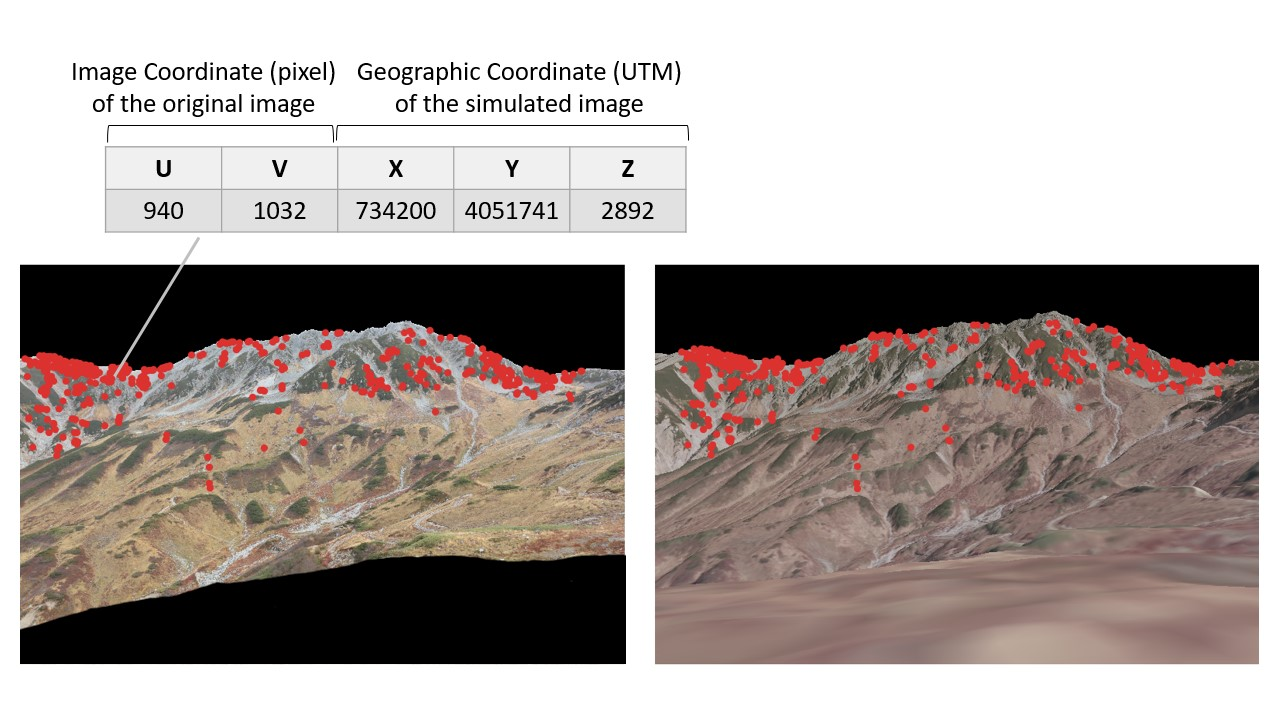
\includegraphics[width=1\linewidth]{paper_files/figures/Slide4} \caption{Automatic acquisition of GCPs. The original image (left) and the simulated image (right). The simulated image was rendered with an orthophoto, DSM, and initial camera parameters. Red points show the matching points. We used these points as GCPs.}\label{fig:matched}
\end{figure}

\hypertarget{camera-parameter-estimation}{%
\subsection{Camera parameter estimation}\label{camera-parameter-estimation}}

The acquired GCPs were used to estimate the camera parameters of the images. By applying the camera model to the geographical coordinates of the GCPs (\(X, Y, Z\) in Fig. \ref{fig:optim}), the reprojected image coordinates can be calculated with a set of camera parameters. The distance from the actual image coordinates of the GCPs (\(U, V\) in Fig. \ref{fig:optim}) to the reprojected image coordinates (\(U', V'\) of Fig. \ref{fig:optim}) can then be measured. We estimated the camera parameters by minimizing this distance using a Covariance Matrix Adaptation Evolution Strategy (CMA-ES, \cite{Hansen2003CMAES}, Fig. \ref{fig:optim}). A CMA-ES performs well in optimizing a complex multimodal function with fewer parameters to be set. We were unable to estimate the camera location as it increased the complication of the problem (e.g., a telephoto taken from a distance and a wide-angle taken from a close look similar).



\begin{figure}
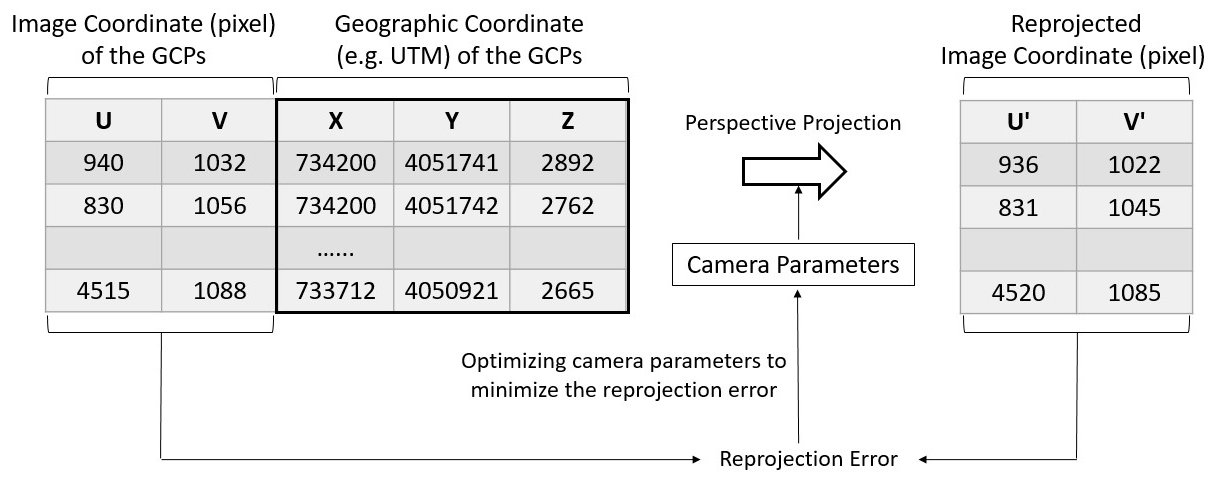
\includegraphics[width=1\linewidth]{paper_files/figures/Slide5} \caption{Workflow of the camera parameter optimization. We estimated the camera parameters by minimizing the GCP's reprojection error.}\label{fig:optim}
\end{figure}

\hypertarget{georectification-of-the-vegetation-map}{%
\subsection{Georectification of the vegetation classification map}\label{georectification-of-the-vegetation-map}}



\begin{figure}
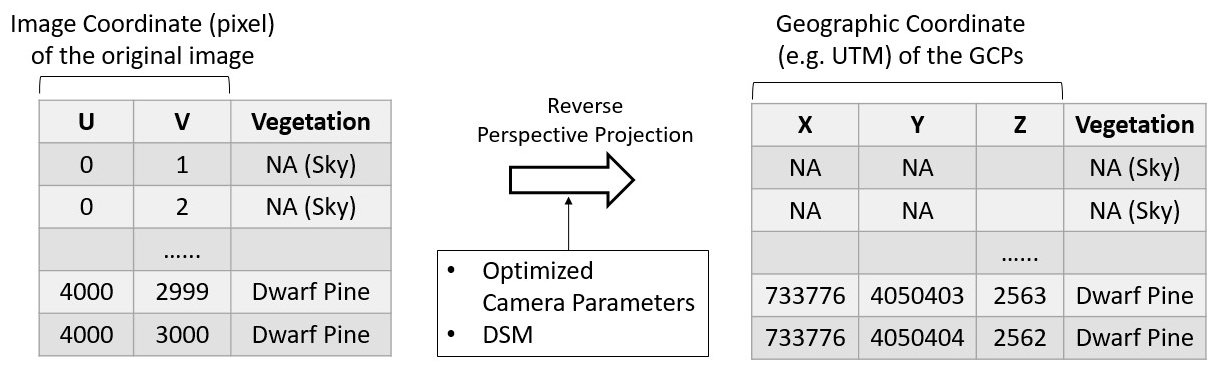
\includegraphics[width=1\linewidth]{paper_files/figures/Slide6} \caption{Our georectification procedure. We applied the optimized camera parameters to the DSM and the vegetation classification result to get a vegetation classification map.}\label{fig:georec}
\end{figure}

Finally, we georectified the vegetation classification results using the optimized camera parameters (Fig. \ref{fig:georec}). At this point, we obtained the point data for the vegetation types(as shown in the table on the right of Fig. \ref{fig:georec}, where every row represents a pixel of the original image). We converted the point data into raster data to measure the area of each vegetation class. We rasterized the point data at a resolution of 1 m and then interpolated holes up to 2 m because the maximum pixel footprint was approximately 2 m on the ridge of the mountain. This rasterization procedure was implemented using the R  (\cite{Rcore}) ``stars''  (\cite{Rstars}) and ``terra'' (\cite{Rterra}) packages. See \url{https://github.com/0kam/VegetationMapPaper/blob/master/scripts/utils/interpolate.R} for the source code.

\hypertarget{implementation-and-evaluation}{%
\subsection{Implementation and evaluation}\label{implementation-and-evaluation}}

We implemented the proposed procedure using Python3 and published it as an open-source package via GitHub (\url{https://github.com/0kam/alproj}). We used an airborne image and DSM in the GCP acquisition process. The Japanese Forestry Agency captured airborne images in the fall of 2010 and orthorectified them using a digital elevation model (DEM) produced by airborne laser scanning. This DEM was also used as the DSM in the GCP acquisition and georectification processes. The airborne image and DSM had spatial resolutions of 0.2 m and 2 m, respectively, and were both resampled to a resolution of 1 m.

The accuracy of the georectification method was tested. We manually searched 83 matching points between the simulated and original images and treated them as test GCPs (i.e., GCPs that were not used in the georectification process). First, we used the silhouette-based matching method (hereafter referred to as the silhouette method) used in the previous study (\cite{Portenier2020Cryosphere})to demonstrate the benefits of the image-matching-based GCP acquisition method. That is, we considered lens distortion in the silhouette, whereas \cite{Portenier2020Cryosphere} did not. Second, our method without the lens distortion model (hereafter referred to as no distortion) was used to evaluate the advantages of the lens distortion model. We evaluated the projection errors of the test GCPs using these three methods.

\hypertarget{results}{%
\section{Results}\label{results}}

\hypertarget{vegetation-classification-accuracy}{%
\subsection{Vegetation classification accuracy}\label{vegetation-classification-accuracy}}



\begin{figure}
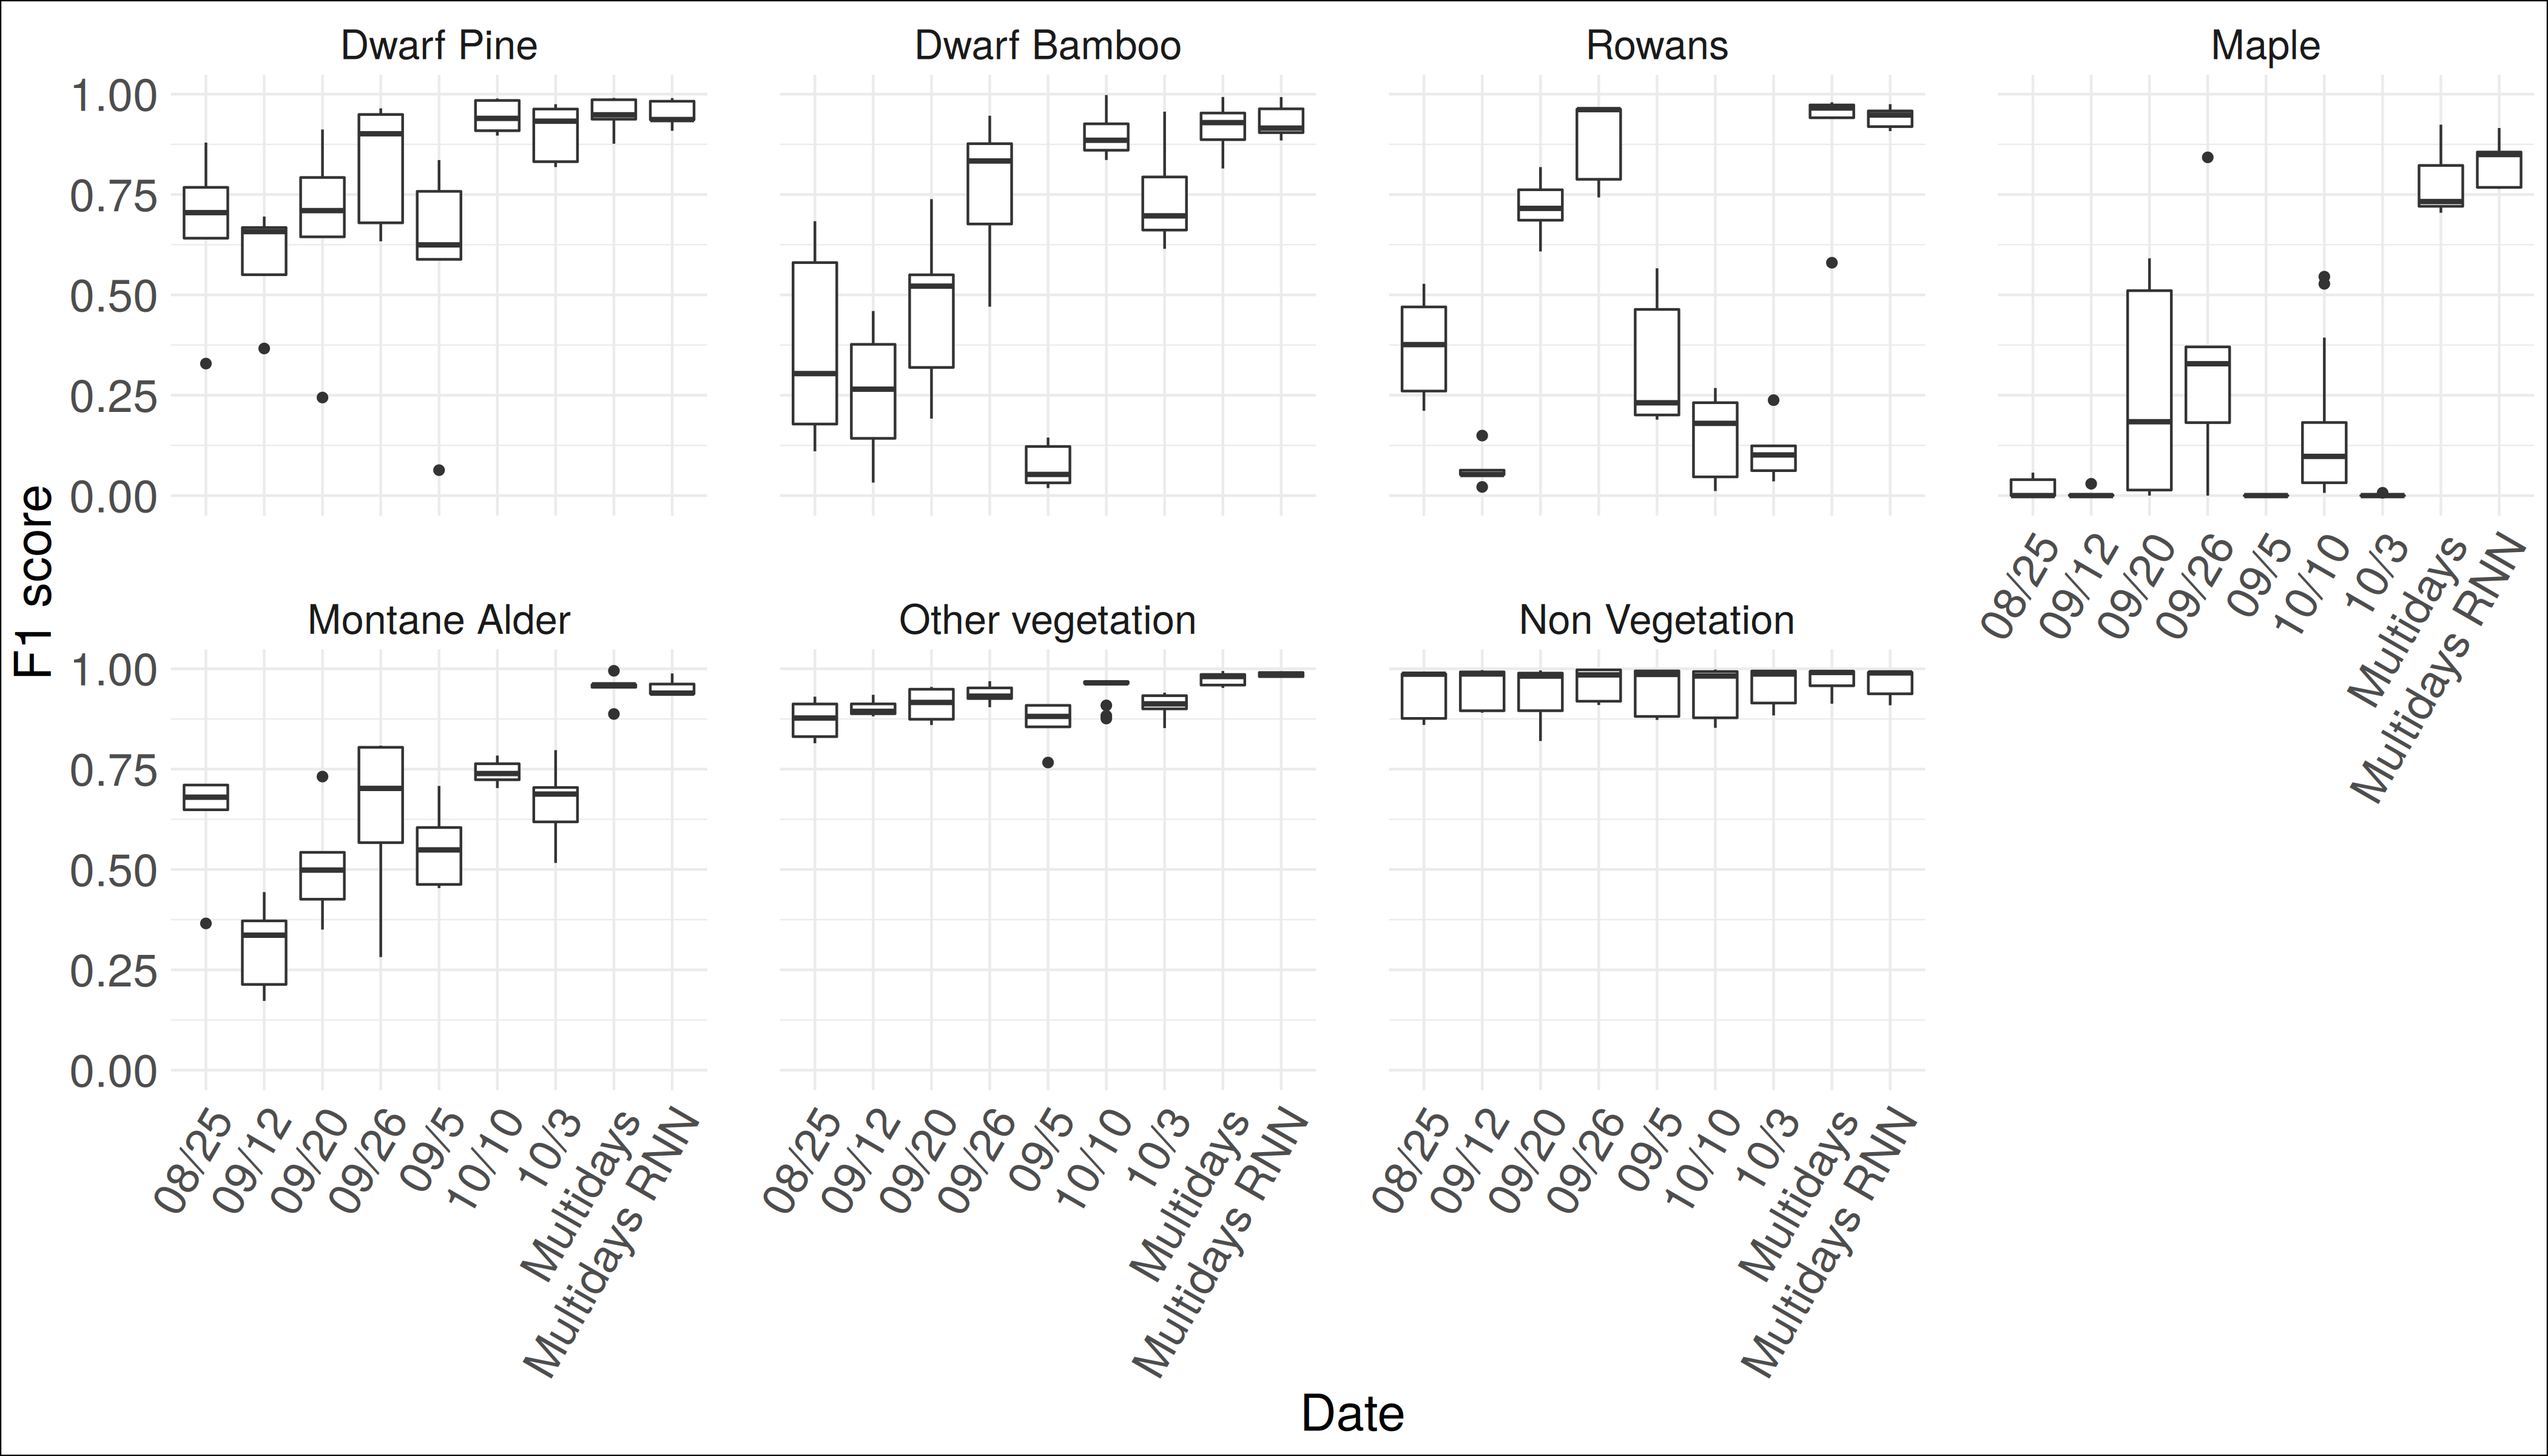
\includegraphics[width=1\linewidth]{paper_files/figures/cv} \caption{The per-class F1-scores of the vegetation classification. Each box plot shows the results of a 5-fold cross-validation. We classified each pixel of a single image (shown as the shooting date) with SVM classifiers, and pixel time series with SVM (shown as ``Multidays'') and RNN (shown as ``Multidays RNN'') classifiers.}\label{fig:vegeacc}
\end{figure}



\begin{figure}
\includegraphics[width=1\linewidth]{paper_files/figures/vege} \caption{Left: Vegetation classification results of the RNN model. The masked area, i.e., the sky and the regions too close to the camera, is shown in black. Right: The generated vegetation classification map. The background shows contour lines.}\label{fig:vegetation}
\end{figure}

Fig. \ref{fig:vegeacc} shows the results of the 5-fold cross-validation. When focusing on a single-day classification (shown as the shooting date), the best classification date differed between classes. For example, September 26 was the best for identifying Rowans, but October 10 was the best for identifying Dwarf Pine and Dwarf Bamboo. The fall colorization of Rowans was best on September 26, and most vegetation (except Dwarf Bamboo and Dwarf Pine) was blasted on October 10. No single image could accurately classify Maple or Montane Alder. In contrast, using all images (shown as ``Multidays'' and ``Multidays RNN'' representing the SVM and RNN classifiers, respectively) resulted in a high F1 score in every class. In addition, the RNN classifier outperformed the SVM classifier ( macro average F1 scores of 0.937 and 0.918, respectively). Fig. \ref{fig:vegetation} (left) shows the products of the RNN classifier. We observed the distribution of each vegetation class at the plant-community scale.

\hypertarget{georectification-accuracy}{%
\subsection{Georectification accuracy}\label{georectification-accuracy}}

The proposed method achieved accurate projection (RMSE = 3.45 m), whereas the other methods did not (RMSE = 16.1 m and 23.6 m using the silhouette and no distortion methods, respectively). We also checked the relationship between the projection error and the distance from the shooting point for each test GCP (Fig. \ref{fig:geoacc})to examine our method's georectification error. The projection error was particularly large in the GCPs near the shooting point. Fig. \ref{fig:vegetation} (right) shows the produced vegetation classification map. The vegetation classification map has missing areas because ridges blocked the view of the camera.

\begin{figure}
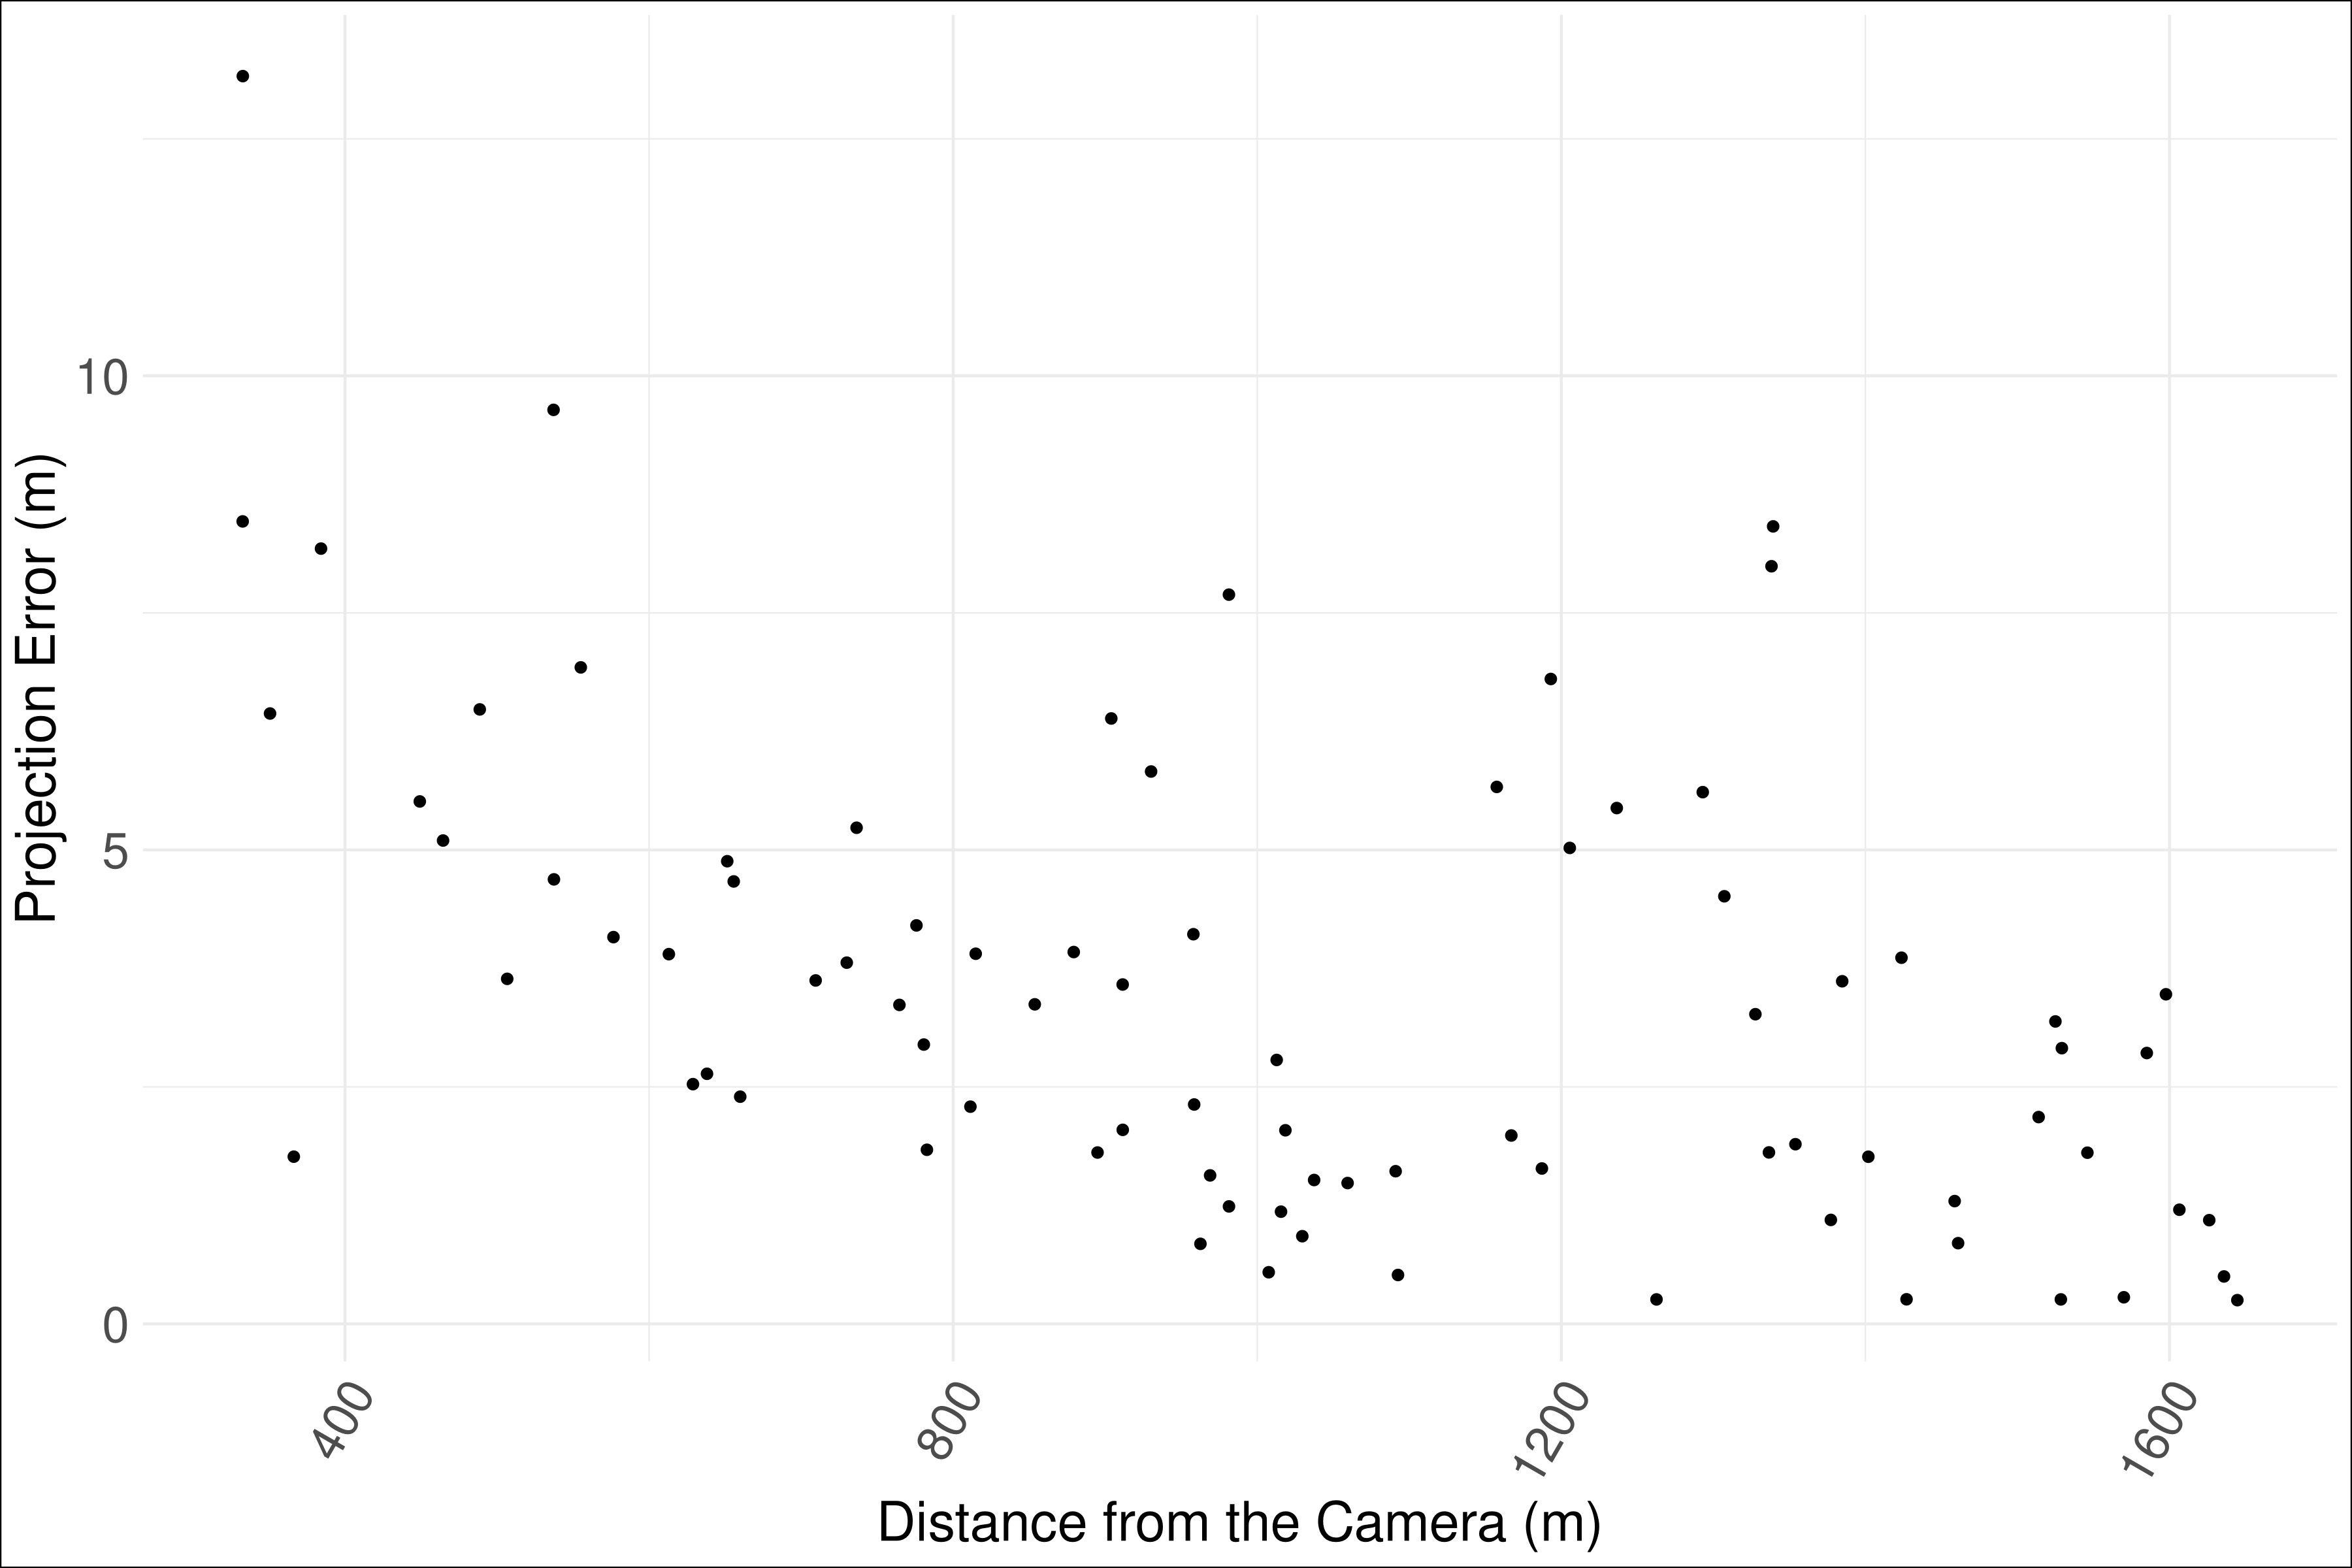
\includegraphics[width=1\linewidth]{paper_files/figures/georec_acc} \caption{The projection error of the proposed method. The projection error was particularly large in the area near the camera.}\label{fig:geoacc}
\end{figure}

\hypertarget{discussion}{%
\section{Discussion}\label{discussion}}

We proposed a low-cost automated procedure to transform time-lapse images of alpine regions into georeferenced vegetation classification maps. Two aspects made this a challenging task: 1) the difficulty of classifying vegetation using ordinal digital camera imagery, and 2) the difficulty of georectifying such ground-based imagery. We solved these issues by: 1) using the temporal information of fall leaf colors for vegetation classification, and 2) developing a novel method for accurate image georectification. The proposed methods performed functionally (0.937 mean F1 Score of vegetation classification and 3.4 m mean projection error of georectification,) and the vegetation classification map could be used in monitoring the vegetation distributions at a plant-community scale.

\hypertarget{the-benefit-of-using-time-series-imagery-for-vegetation-classification}{%
\subsection{The benefit of using time-series imagery for vegetation classification}\label{the-benefit-of-using-time-series-imagery-for-vegetation-classification}}

One of the shortcomings of ordinary digital cameras is that they have only three bands (Red, Blue, and Green). We compensated for this lack of information by using the rich temporal information that time-lapse data collection offers. Many plant species have characteristic phenologies, such as fall foliage, and the suitable season to observe them differs among species. The accuracy of the single-day classification (see shooting dates in Fig. \ref{fig:vegeacc}) shows that the best time for identification from the images varied with vegetation class. Classifying multiple vegetation classes requires long-term (e.g., several months) and frequent (such as daily) monitoring, and digital time-lapse cameras are suitable for this purpose. In addition, combining multitemporal images improved the classification accuracy, especially for Maple and Montane Alder. The best F1 score achieved using the single-day classification was low (0.750 for Montane Alder, 0.345 for Maple), whereas it was improved significantly (0.951 and 0.781 with the SVM classifier) by using multitemporal images. This shows that identifying these classes requires multitemporal information. As indicated in a previous study (\cite{Ienco2017RemSenLSTMn the RNN model outperformed the SVM model. This result was particularly noticeable for Maple (0.781 with SVM and 0.831 with RNN), which exhibited intraspecies variation in fall foliage timings. We found a weak correlation between two Maple pixel time series with different fall foliage timings but a strong temporal correlation. This may explain why the SVM model could not correctly detect Maple: it ignores the temporal correlation of the data, while the RNN model does not. However, our model can still be improved further. As (\cite{Sharma2018NN}) claimed, patch-based classification methods may improve performance. Such patch-based models use a time series of small patches as input to utilize the spatial information, such as textures, in the classification process.

\hypertarget{the-performance-of-the-georectification-method-and-its-limitation.}{%
\subsection{The performance of the georectification method and its limitation.}\label{the-performance-of-the-georectification-method-and-its-limitation.}}

The most significant barrier to using ground-based imagery in ecological monitoring is the difficulty of treating it as geospatial data. Therefore, an automated and accurate georectification method is required to overcome this challenge. Without georectification, we cannot quantitatively analyze (e.g., measure the area, locate the place, or analyze the topographic data) the acquired information, such as vegetation distribution. We propose a novel method to georectify such imagery. With minimal manual user inputs (i.e., the camera location and initial camera parameters), our approach achieved a very high level of accuracy (3.45 m). We tested the effectiveness of two features of our method: the lens distortion model and the image-matching-based method for acquiring GCPs.

The results demonstrate that the lens distortion model significantly improved the georectification accuracy. Without the lens distortion model, our model resulted in a projection accuracy of 23.6 m. However, as the effect of lens distortion on the georectification accuracy is different among cameras and lenses (\cite{Portenier2020Cryosphere}), further testing will be required. Another feature of our method is the automatic acquisition of GCPs using simulated images and image-matching techniques. A high-resolution orthophoto that covers the field of view of the camera is required. This is quite expensive, but the reward is considerable. The conventional silhouette-based method resulted in an RMSE of 16.1 m. This suggests that acquiring matching points between the image and DSM in a broader area benefits the camera parameter estimation process. 

However, our method has some limitations. The proposed lens distortion model does not support a fisheye lens or omnidirectional camera. Focusing on the GCP acquisition method, we assumed that the landscape (e.g., topography and vegetation cover) would appear the same between the original and simulated images. While we employed a robust matching method, significant changes in the mountain terrain (such as those caused by landslides) may cause a matching error. Slight changes in vegetation cover may also affect the quality of the GCPs. However, the negative effect (a few meters) of using these points as GCPs should be much smaller than the positive effect (approximately 12.6 m). In addition, the AKAZE image matcher could not acquire matching points in the area near the camera, and here the projection error was relatively large (Fig. \ref{fig:geoacc}). While the spatial resolution of the simulated image depends on the orthophoto and is constant (in this study, 1 m), that of the original image changes depending on the distance from the camera. In areas near the camera, the spatial resolution of the original image is much higher than that of the simulated image, and the image matcher cannot handle this difference. Recently, researchers developed deep-learning-based image-matching methods (e.g., \cite{Yang2018ImageMatching}, \cite{Wu2013AEImageMatching}) that are more robust in terms of differences in image sources and viewpoints. Applying these methods to the GCP acquisition process may improve the performance of our method, especially in nearby areas. 

Theoretically, our approach can handle images of other ecosystems, such as forests. However, this may be difficult because georectification accuracy strongly depends on the accuracy of the DSM. Because alpine plants tend to be very short, readily available Digital Elevation Models (DEMs) can be used as DSMs. In forestry areas, vegetation height is considerable, and the gap between the DEMs and the actual surface (top of the forest) may cause significant errors in the georectification process.

\hypertarget{future-application-and-conclusion}{%
\subsection{Future application and conclusion}\label{future-application-and-conclusion}}

In this study, we propose an automated method to draw a vegetation classification map from a series of images acquired using a digital time-lapse camera. The vegetation classification map had sufficient accuracy for monitoring endemic and vulnerable alpine vegetation. One benefit of digital time-lapse cameras is their long-term operability. Applying the proposed method to existing long-term time-lapse imagery will enable researchers to quantitatively understand vegetation changes and their trends. This information will help researchers and stakeholders plan field observations and conservation activities more effectively. Our methods facilitate cost-efficient monitoring of alpine vegetation and understanding the impacts of climate change on alpine ecosystems.

%TC:ignore
\hypertarget{acknowledgement}{%
\section*{Acknowledgement}\label{acknowledgement}}
The authors would like to thank Tohru Ohmiya and Hisashi Sugita for their help with field observations and validation of the training dataset.
%TC:endignore

\bibliographystyle{unsrt}
\bibliography{export.bib}


\end{document}

